\documentclass[10pt,twocolumn]{article}

% --- Page layout ---
\usepackage[a4paper,margin=1.7cm]{geometry}
\setlength{\columnsep}{0.6cm}

% --- Font & micro-typography ---
\usepackage{newtxtext,newtxmath}
\usepackage[final]{microtype}

% --- Graphics, floats, tables ---
\usepackage{graphicx}
\usepackage{booktabs}
\usepackage{siunitx}
\sisetup{detect-all, group-separator={,}, group-minimum-digits=4}
\usepackage[font=small,labelfont=bf]{caption}
\usepackage{subcaption}
\usepackage{float}   % for [H] placement
\usepackage{xspace}
\usepackage{xcolor}

% --- Math & refs ---
\usepackage{amsmath,amssymb}
\usepackage[hidelinks]{hyperref}
\usepackage[capitalise,nameinlink]{cleveref}

% --- References ---
\usepackage[
    backend=biber,    % modern backend
    style=authoryear, % or numeric, apa, etc.
    maxbibnames=6,    % number of names shown before et al.
    doi=false,isbn=false,url=false,eprint=false % trim fields
]{biblatex}

\addbibresource{references.bib} 

% --- Tighten spacing ---
\setlength{\textfloatsep}{6pt plus 2pt minus 2pt}
\setlength{\intextsep}{6pt plus 2pt minus 2pt}
\setlength{\abovecaptionskip}{4pt}
\setlength{\belowcaptionskip}{0pt}
\setlength{\abovedisplayskip}{6pt}
\setlength{\belowdisplayskip}{6pt}
\pagestyle{empty}

% --- Handy macros ---
\newcommand{\todo}[1]{\textcolor{red}{[#1]}}
\newcommand{\codeurl}{\url{https://example.com/repo}\xspace}
\newcommand{\dataurl}{\url{https://example.com/data}\xspace}

% zero-dependency placeholder figure
\newcommand{\placeholderfig}[1][48mm]{\fbox{\parbox[c][#1][c]{\linewidth}{\centering Placeholder figure}}}

\title{\vspace{-6pt}\textbf{Sparse Signals in Stock Returns and News}\vspace{-4pt}}

\date{}

\begin{document}
\maketitle
\vspace{-18pt}

\begin{abstract}
\noindent
We generate one-day-ahead return forecasts for the full universe of S\&P 500 stocks using two sets of predictors: (i) lagged returns of all index stocks and (ii) estimates of news attention to business and finance topics. We follow \cite{chinco2019sparse} and employ the Least Absolute Shrinkage and Selection Operator (LASSO). This approach allows us to handle a high-dimensional predictor set with relatively few observations by shrinking most coefficients to zero and retaining only a sparse subset of predictive signals. 
Our results show that (i) the number of selected predictors decreases monotonically with the penalty parameter $\lambda$, which tends to rise during volatile periods, (ii) combining the LASSO forecast with an AR(3) benchmark explains on average an additional 2.1\% of daily return variation, and (iii) only about 7\% of selected predictors exhibit time-series persistence, with higher persistence during episodes of market stress such as the COVID-19 crash.
\end{abstract}

\section{Data}
\label{sec:data}

\textbf{Stocks.} We use all daily stock returns for firms in the S\&P 500 over the period from December 28, 2015 to April 3, 2020. The data are obtained from CRSP using the PERMNO identifiers of the constituent firms. Returns $r_{i,t}$ are measured close-to-close.\\
\textbf{News.} Our text corpus consists of 69{,}612 news articles collected from the \emph{New York Times}, \textit{Reuters}, and \textit{CNBC}. Articles are selected using finance-related keywords such as ``stock market'' and ``financial market,'' to ensure relevance to asset pricing. The resulting documents are sent through a standard text processing pipeline. We estimate a Latent Dirichlet Allocation (LDA) model with $K=20$ topics on this corpus. For each day $t$, we aggregate topic shares from articles to construct measures of daily topic attention. We extract AR(1) innovations from the daily topic share data. The resulting series captures unexpected shifts in attention to each topic.

\begin{table}[H]
  \centering
  \caption{Summary statistics for returns and news}
  \label{tab:summstats}
  \setlength{\tabcolsep}{3pt}
  \renewcommand{\arraystretch}{1.05}
  \small
  \resizebox{\columnwidth}{!}{%
  \begin{tabular}{lcccccc}
    \toprule
    {Variable} & {n} & {mean} & {sd} & {q05} & {median} & {q95} \\
    \midrule
    Return & 484 & 0.0004 & 0.0213 & -0.0282 & 0.00087 & 0.0264  \\
    News  &  20 & 0.00004 & 0.0239 & -0.0305 & -0.003973 & 0.0444 \\
    \bottomrule
  \end{tabular}%
  }
\end{table}


\section{Econometric Setup}
\label{sec:setup}

\textbf{Forecast specification.} 
We study whether lagged stock returns and topic-attention 
can forecast one-day-ahead returns. For firm $i$ on day $t$, the forecasting equation is
\begin{align}
r_{i,t+1} 
  &= \alpha_t + \mathbf{R}_{i,t}^{\!\top}\boldsymbol{\delta} 
     + \mathbf{T}_{i,t}^{\!\top}\boldsymbol{\beta} 
     + \varepsilon_{i,t+1}, 
\label{eq:lasso}
\end{align}
where $\mathbf{R}_{i,t}$ is a vector of lagged stock returns, $\mathbf{T}_{i,t}$ is a vector of lagged topic-attention, and $\varepsilon_{i,t+1}$ is the one-day-ahead forecast error.

\textbf{Variable Selection.} 
At each forecast date, the predictor set includes three daily lags of all S\&P 500 stock returns and three lags of all $K=20$ topic-attention variables. We would need to estimate $1561$ parameters for each forecast. To estimate this using OLS we would need at least 1,561 observations per forecast date, which is impossible given that we only observe 1075 trading days. Even if we would have enough data, an OLS specification would not capture short-lived predictors but only those that are significant for longer. This motivates our use of LASSO regularization to perform automatic variable selection. In particular, we estimate the LASSO on a rolling window of $L=30$ days. The optimization problem is then the following: 

\begin{align}
(\hat{\boldsymbol{\delta}}_t,\hat{\boldsymbol{\beta}}_t)
&= \arg\min_{\boldsymbol{\delta},\,\boldsymbol{\beta}}
\Bigg\{
\frac{1}{L}\sum_{\tau=t-L+1}^{t-1}\sum_{i=1}^{N}
\big(r_{i,\tau+1}-\alpha_t-\mathbf{R}_{i,\tau}^{\!\top}\boldsymbol{\delta}-\mathbf{T}_{i,\tau}^{\!\top}\boldsymbol{\beta}\big)^2 \nonumber\\
&\qquad\qquad
+ \lambda\big(\|\boldsymbol{\delta}\|_1+\|\boldsymbol{\beta}\|_1\big)
\Bigg\}.
\label{eq:lasso_opt}
\end{align}

We employ 10-fold cross-validation to choose the penalty parameter $\lambda$ at each iteration. The set of variables selected by equation (\ref{eq:lasso_opt}) is then used to compute the day-ahead return forecast for stock $i$ using equation (\ref{eq:lasso}). \\ Specifically, our rolling window procedure works as follows: We estimate the LASSO using observations from days $t-29$ through $t$, let the LASSO select the optimal subset of predictors for stock $i$, and generate a return forecast for stock $i$ on day $t+1$ using the selected predictors. We then advance the window by one day, re-estimate the model using days $t-28$ through $t+1$, and forecast returns for day $t+2$. This process continues until we reach the end of our sample period. We perform this procedure for all stocks in our sample.

\section{Results}
\label{sec:results}

Figure~\ref{fig:var_selec} plots the penalization parameter $\lambda$ for each one-day-ahead 
forecast against the number of variables selected by the LASSO. As expected, the number of 
non-zero predictors decreases monotonically as $\lambda$ increases. 

Figure~\ref{fig:lambda_avg} reports the average daily value of $\lambda$. The penalty parameter 
varies substantially over time and tends to be higher during periods of elevated market volatility. 
This likely reflects the fact that, in such periods, the LASSO can exploit greater cross-sectional 
variation in returns and news topic attention.

\begin{figure}[h!] % h! means "place here, if possible"
    \centering
    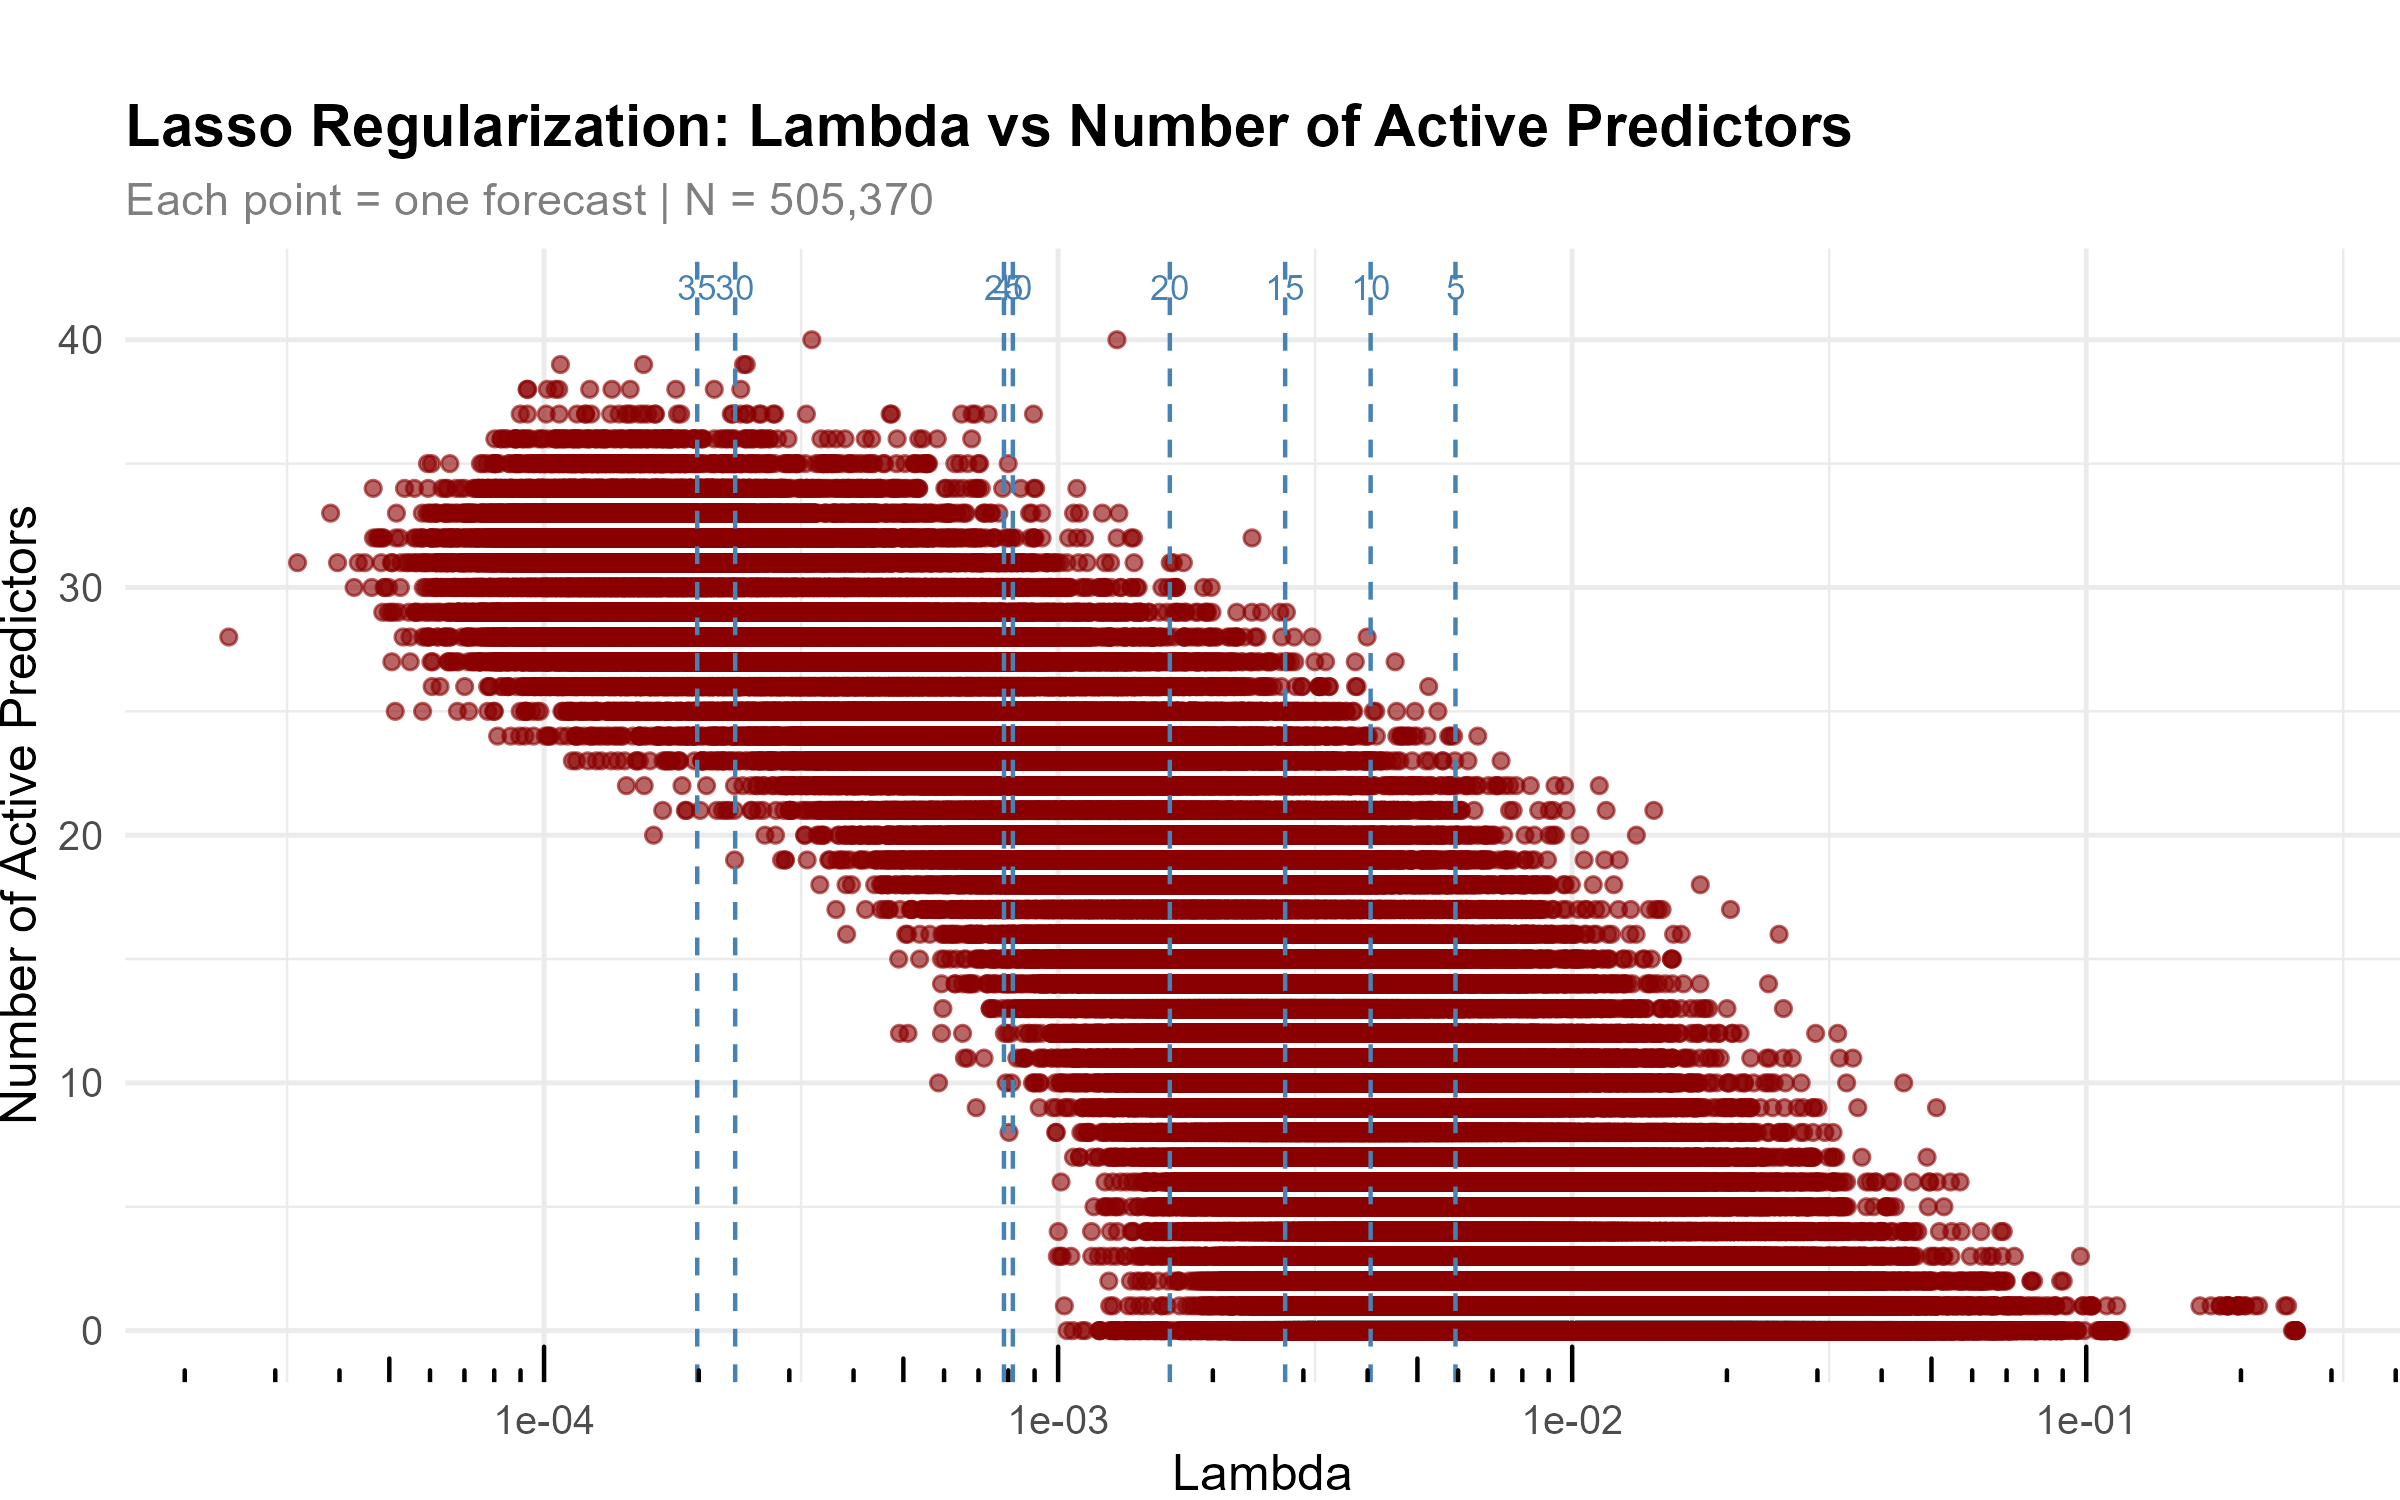
\includegraphics[width=0.45\textwidth]{lambdavspredictors.png} 
    \caption{Number of predictors selected by LASSO as a function of $\lambda$.}
    \label{fig:var_selec} % Label for referencing
\end{figure}

\begin{figure}[h!] % h! means "place here, if possible"
    \centering
    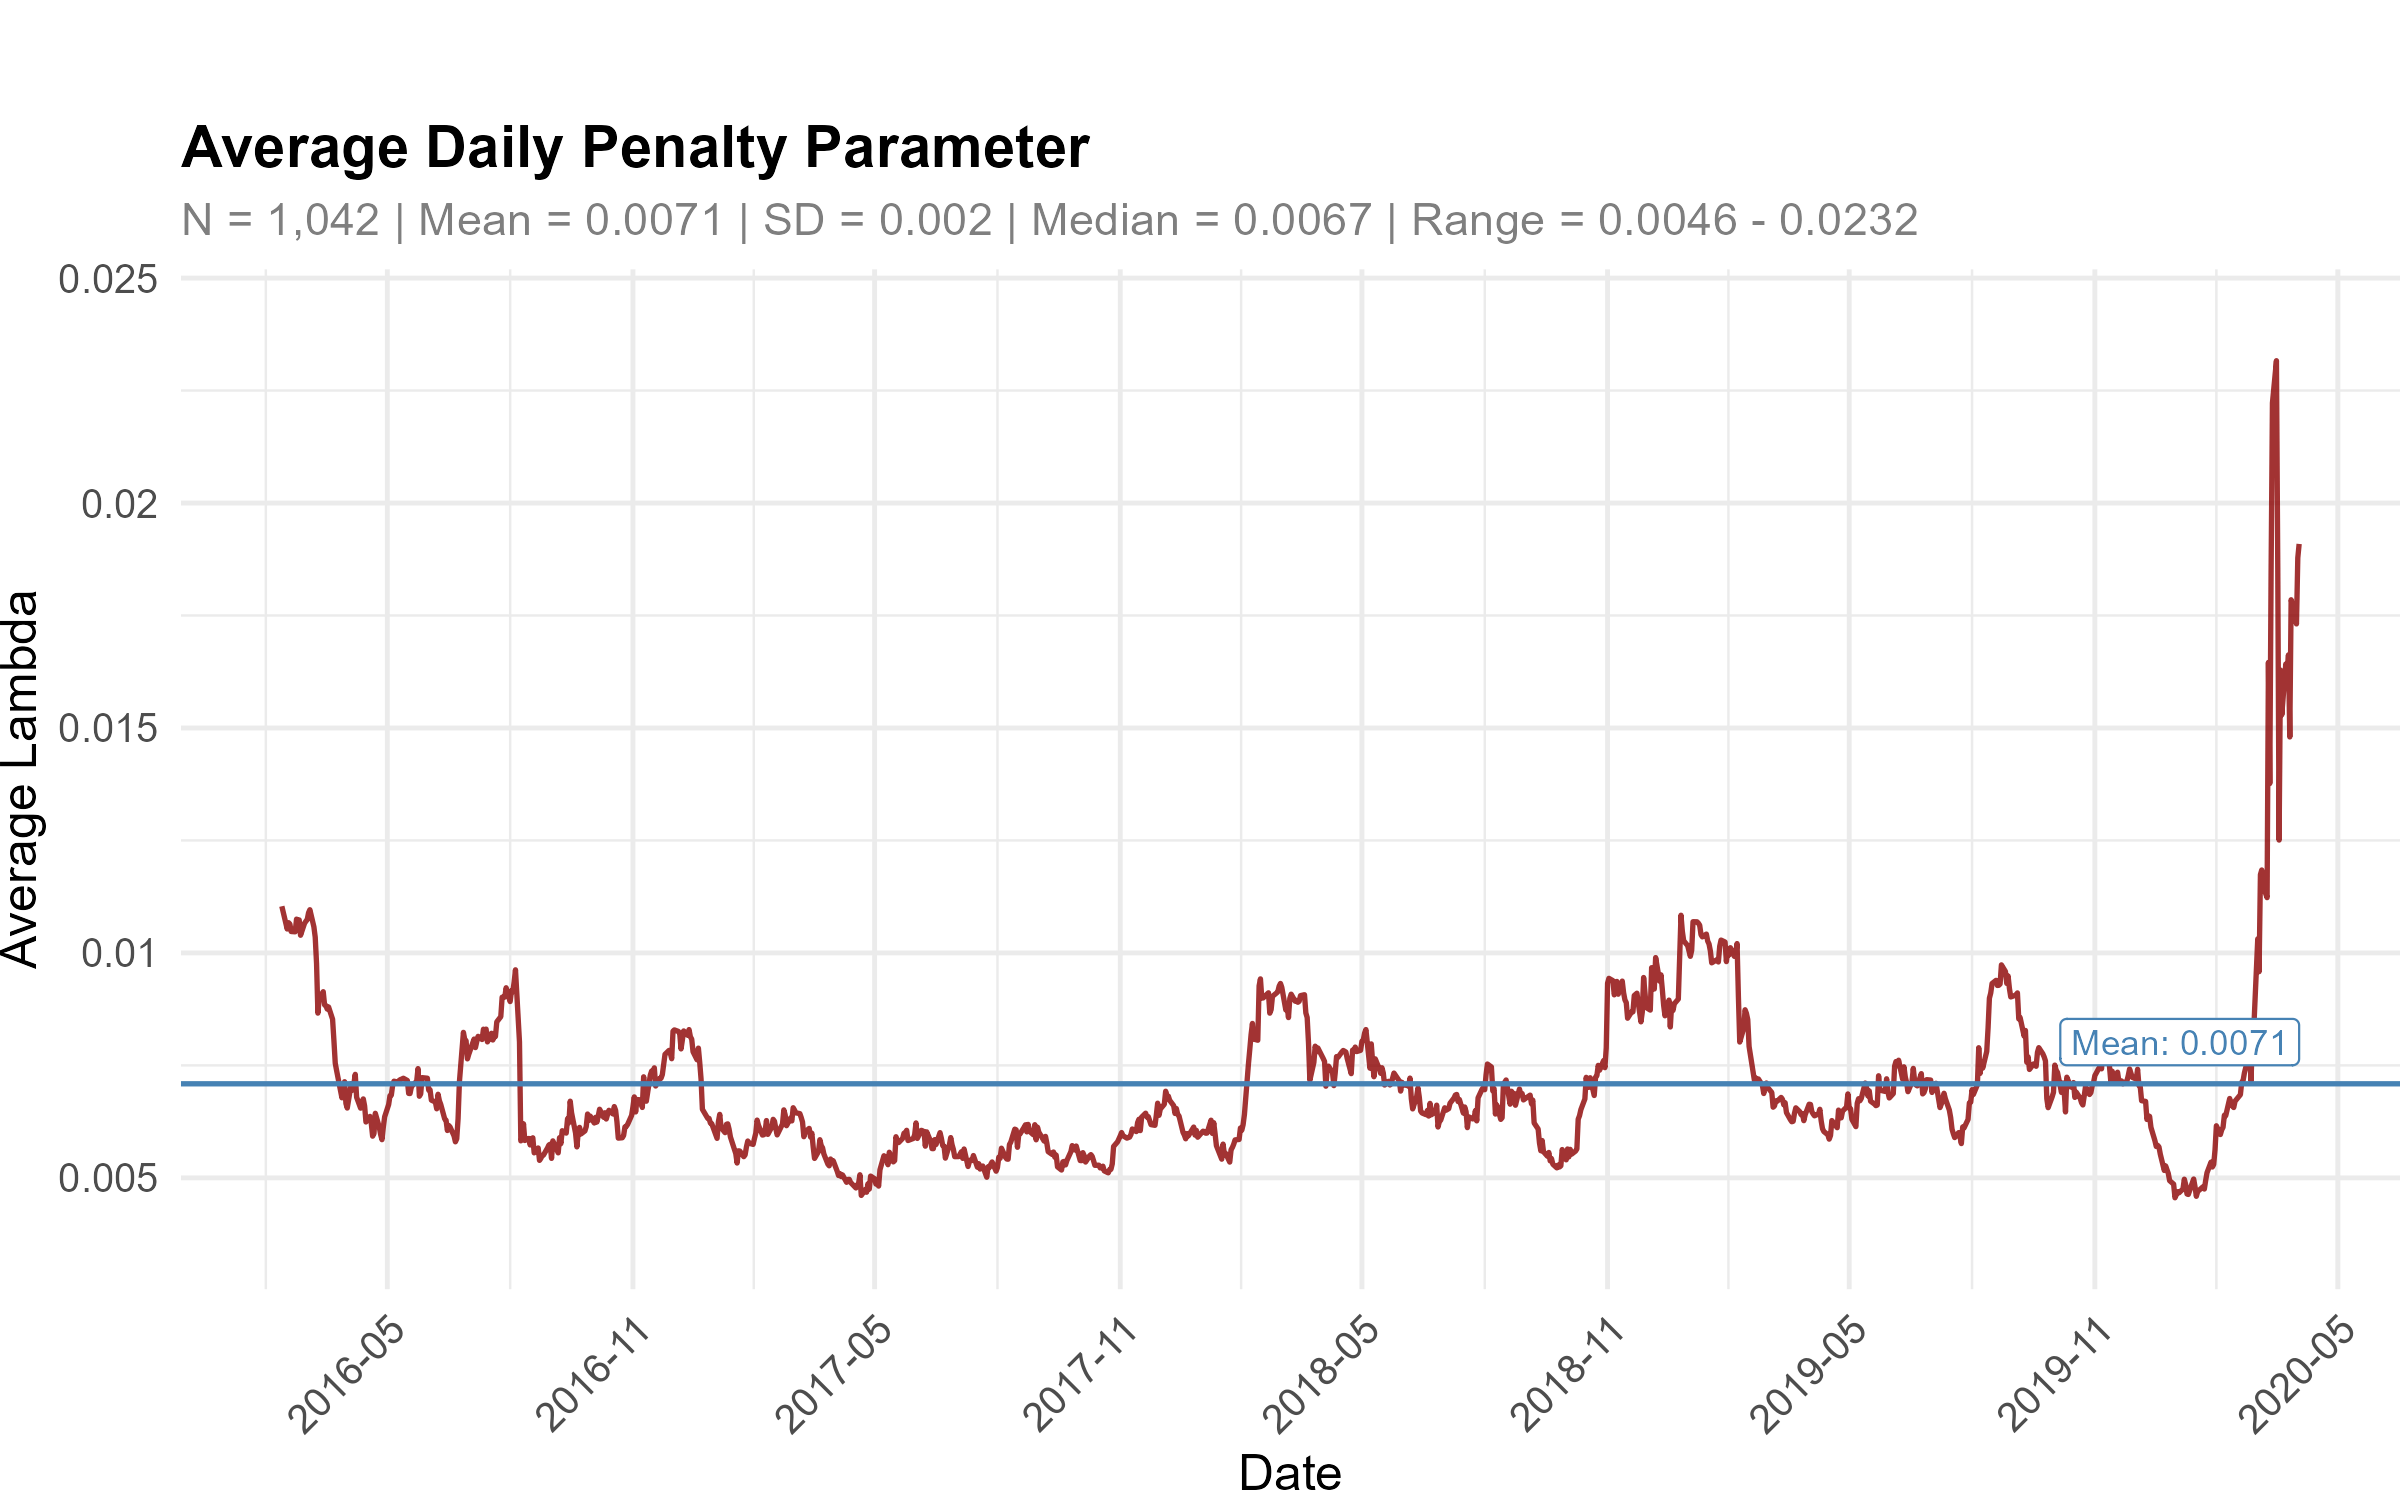
\includegraphics[width=0.45\textwidth]{p_daily_lambda.png} 
    \caption{Average Daily Penalty Parameter $\lambda$.}
    \label{fig:lambda_avg} % Label for referencing
\end{figure}

Next, we assess the degree to which the LASSO forecasts capture the daily cross-sectional variation in individual stock returns. Following \cite{chinco2019sparse}, we estimate the stock-level regression model:  

\begin{align}
r_{i,t} &= \alpha_i + \beta_i z_{i,t} + \varepsilon_{i,t}, \label{eq:r2_reg} \\
z_{i,t} &= \frac{f_{i,t} - \mu_i}{\sigma_i}, \label{eq:standardization}
\end{align}

where \( r_{i,t} \) denotes the realized return of stock \( i \) on day \( t \), and \( f_{i,t} \) is the corresponding one-day-ahead forecast. Each forecast is standardized by subtracting its in-sample mean (\(\mu_i\)) and dividing by its in-sample standard deviation (\(\sigma_i\)). This normalization ensures that regression coefficients are directly comparable across stocks and forecasting models.  

Figures~\ref{fig:r2_oos_lasso} and \ref{fig:r2_oos_benchmark} present the \(R^2\) values from equation~\eqref{eq:r2_reg}, using \(z_{i,t}\) constructed from the LASSO forecasts and, for comparison, from an autoregressive AR(3) benchmark estimated with the same rolling window procedure. On average, the LASSO forecasts explain 1.9\% of the daily variation in returns, outperforming the AR(3) benchmark, which accounts for only 0.8\%.  

\begin{figure}[h!]  
    \centering
    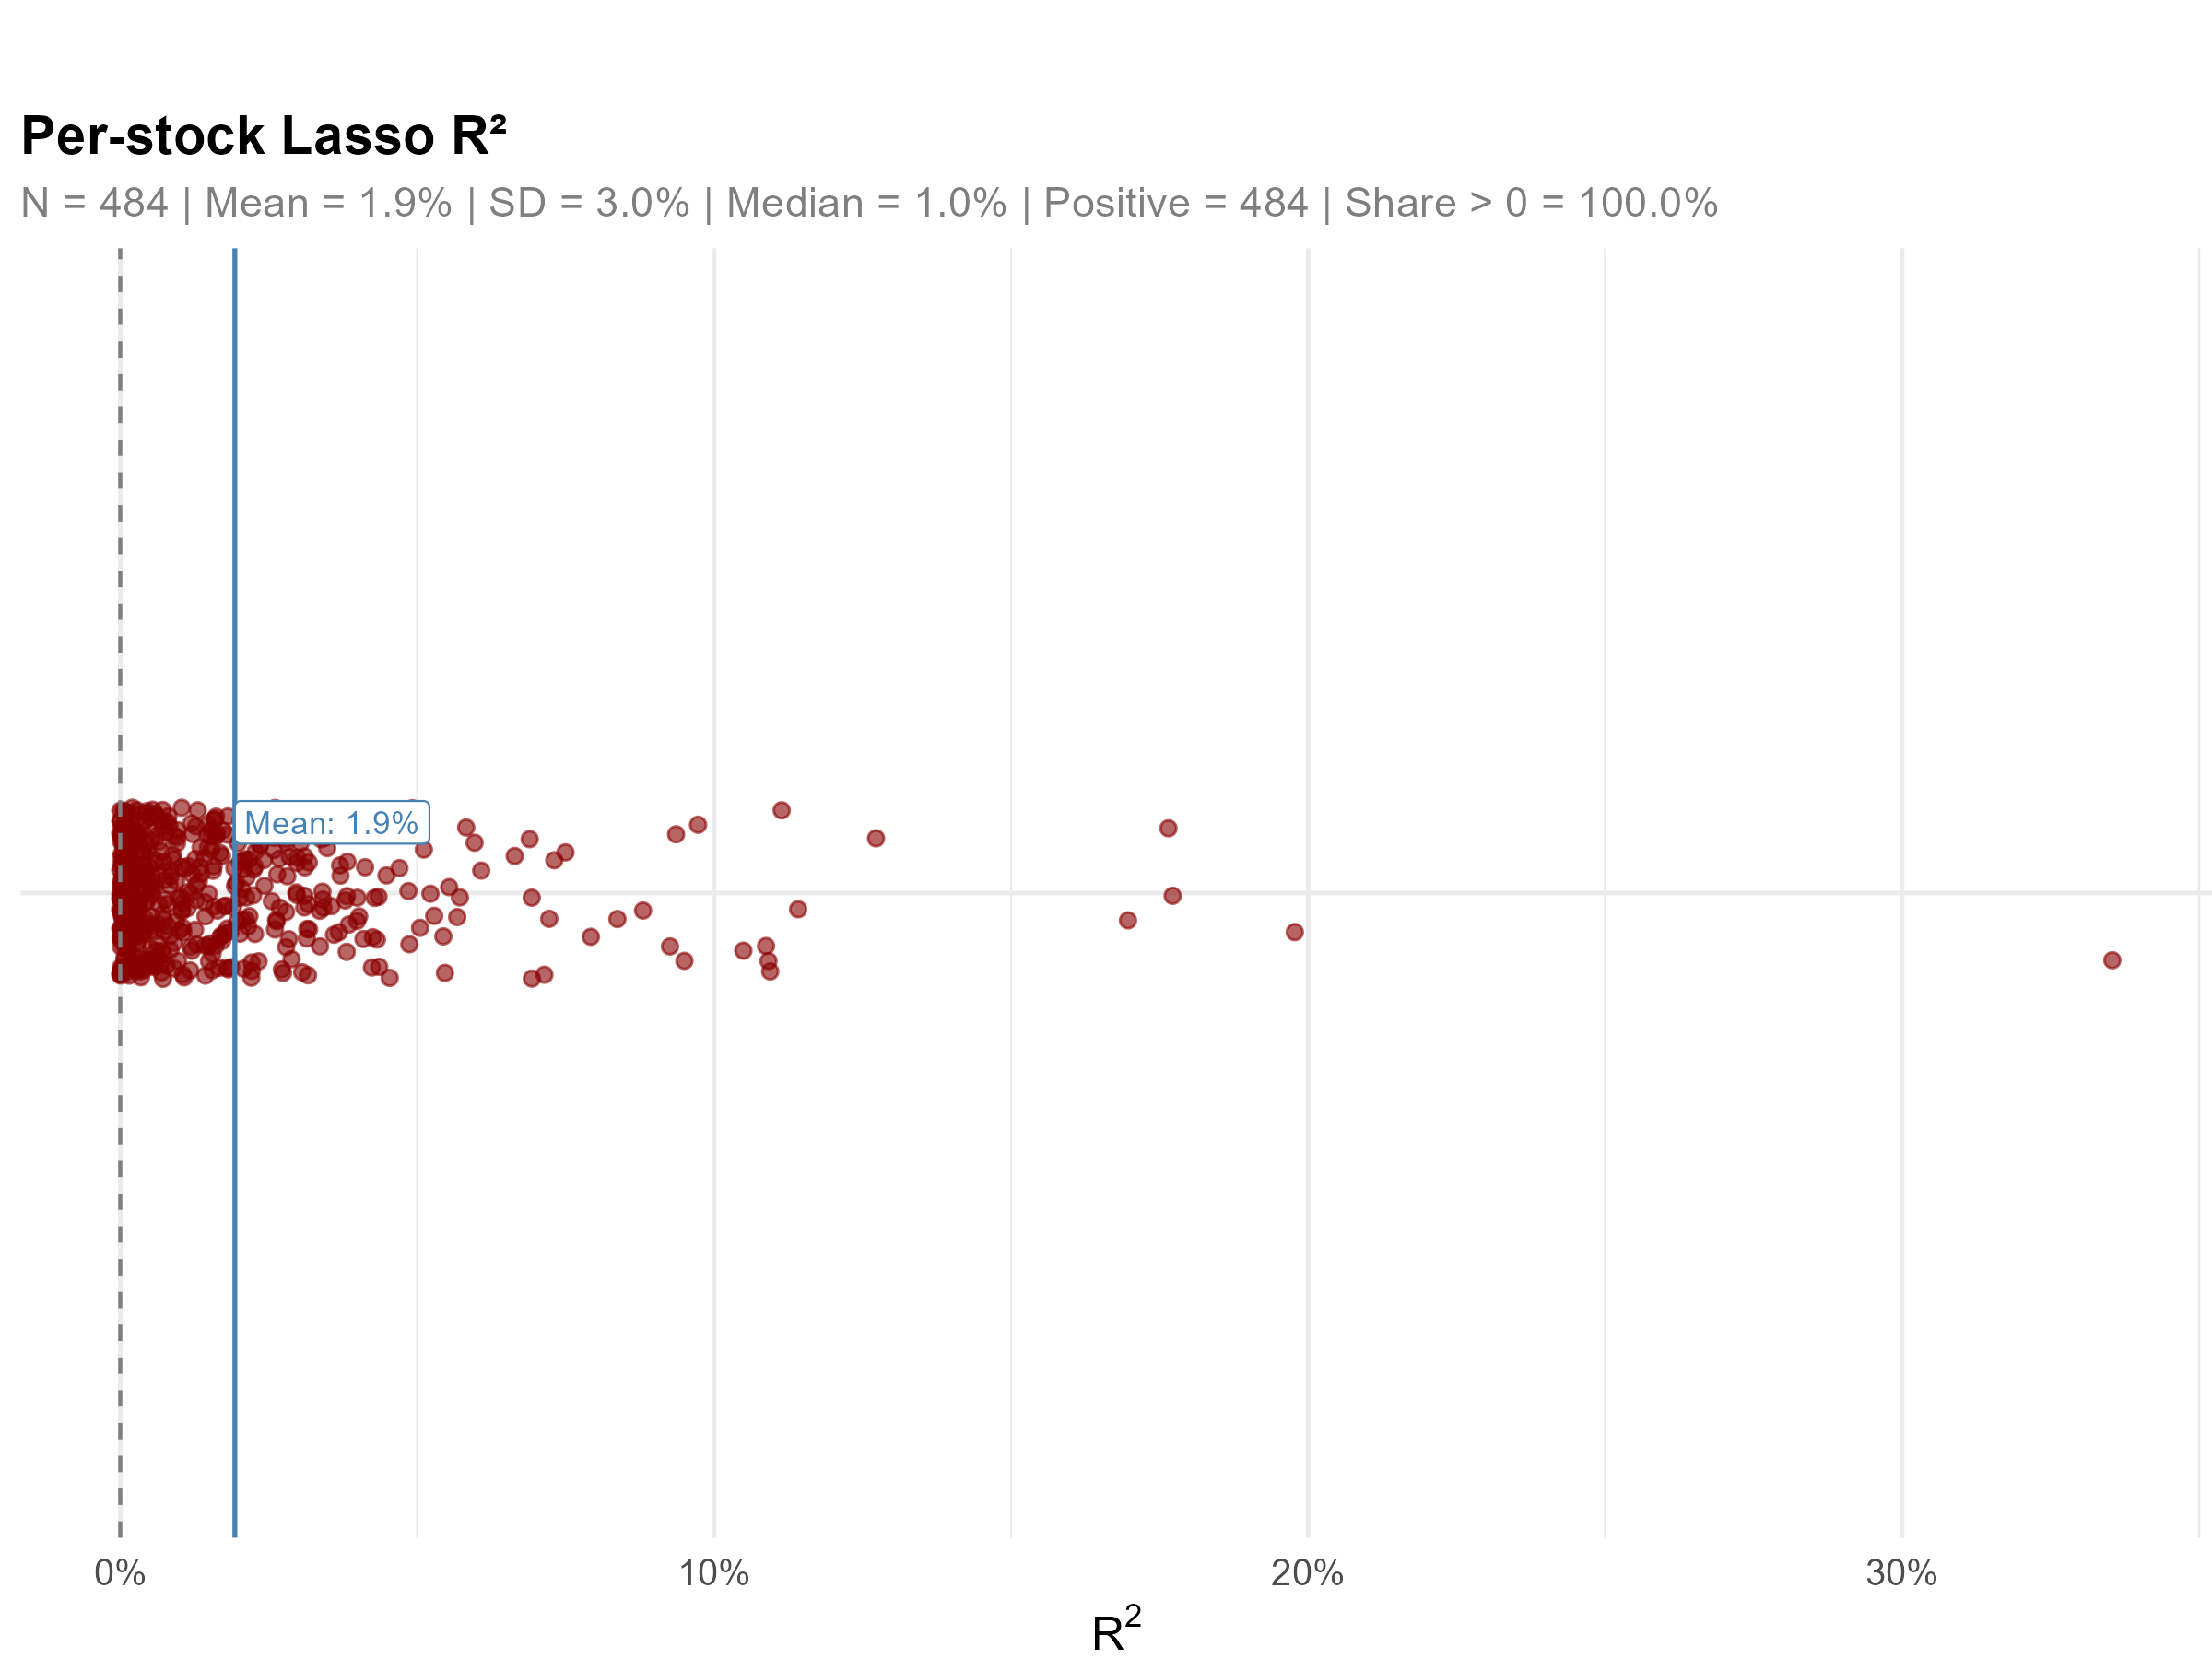
\includegraphics[width=0.45\textwidth]{lasso_r2_plot.png} 
    \caption{\(R^2\) values from regressions using LASSO forecasts.}
    \label{fig:r2_oos_lasso}  
\end{figure}

\begin{figure}[h!]  
    \centering
    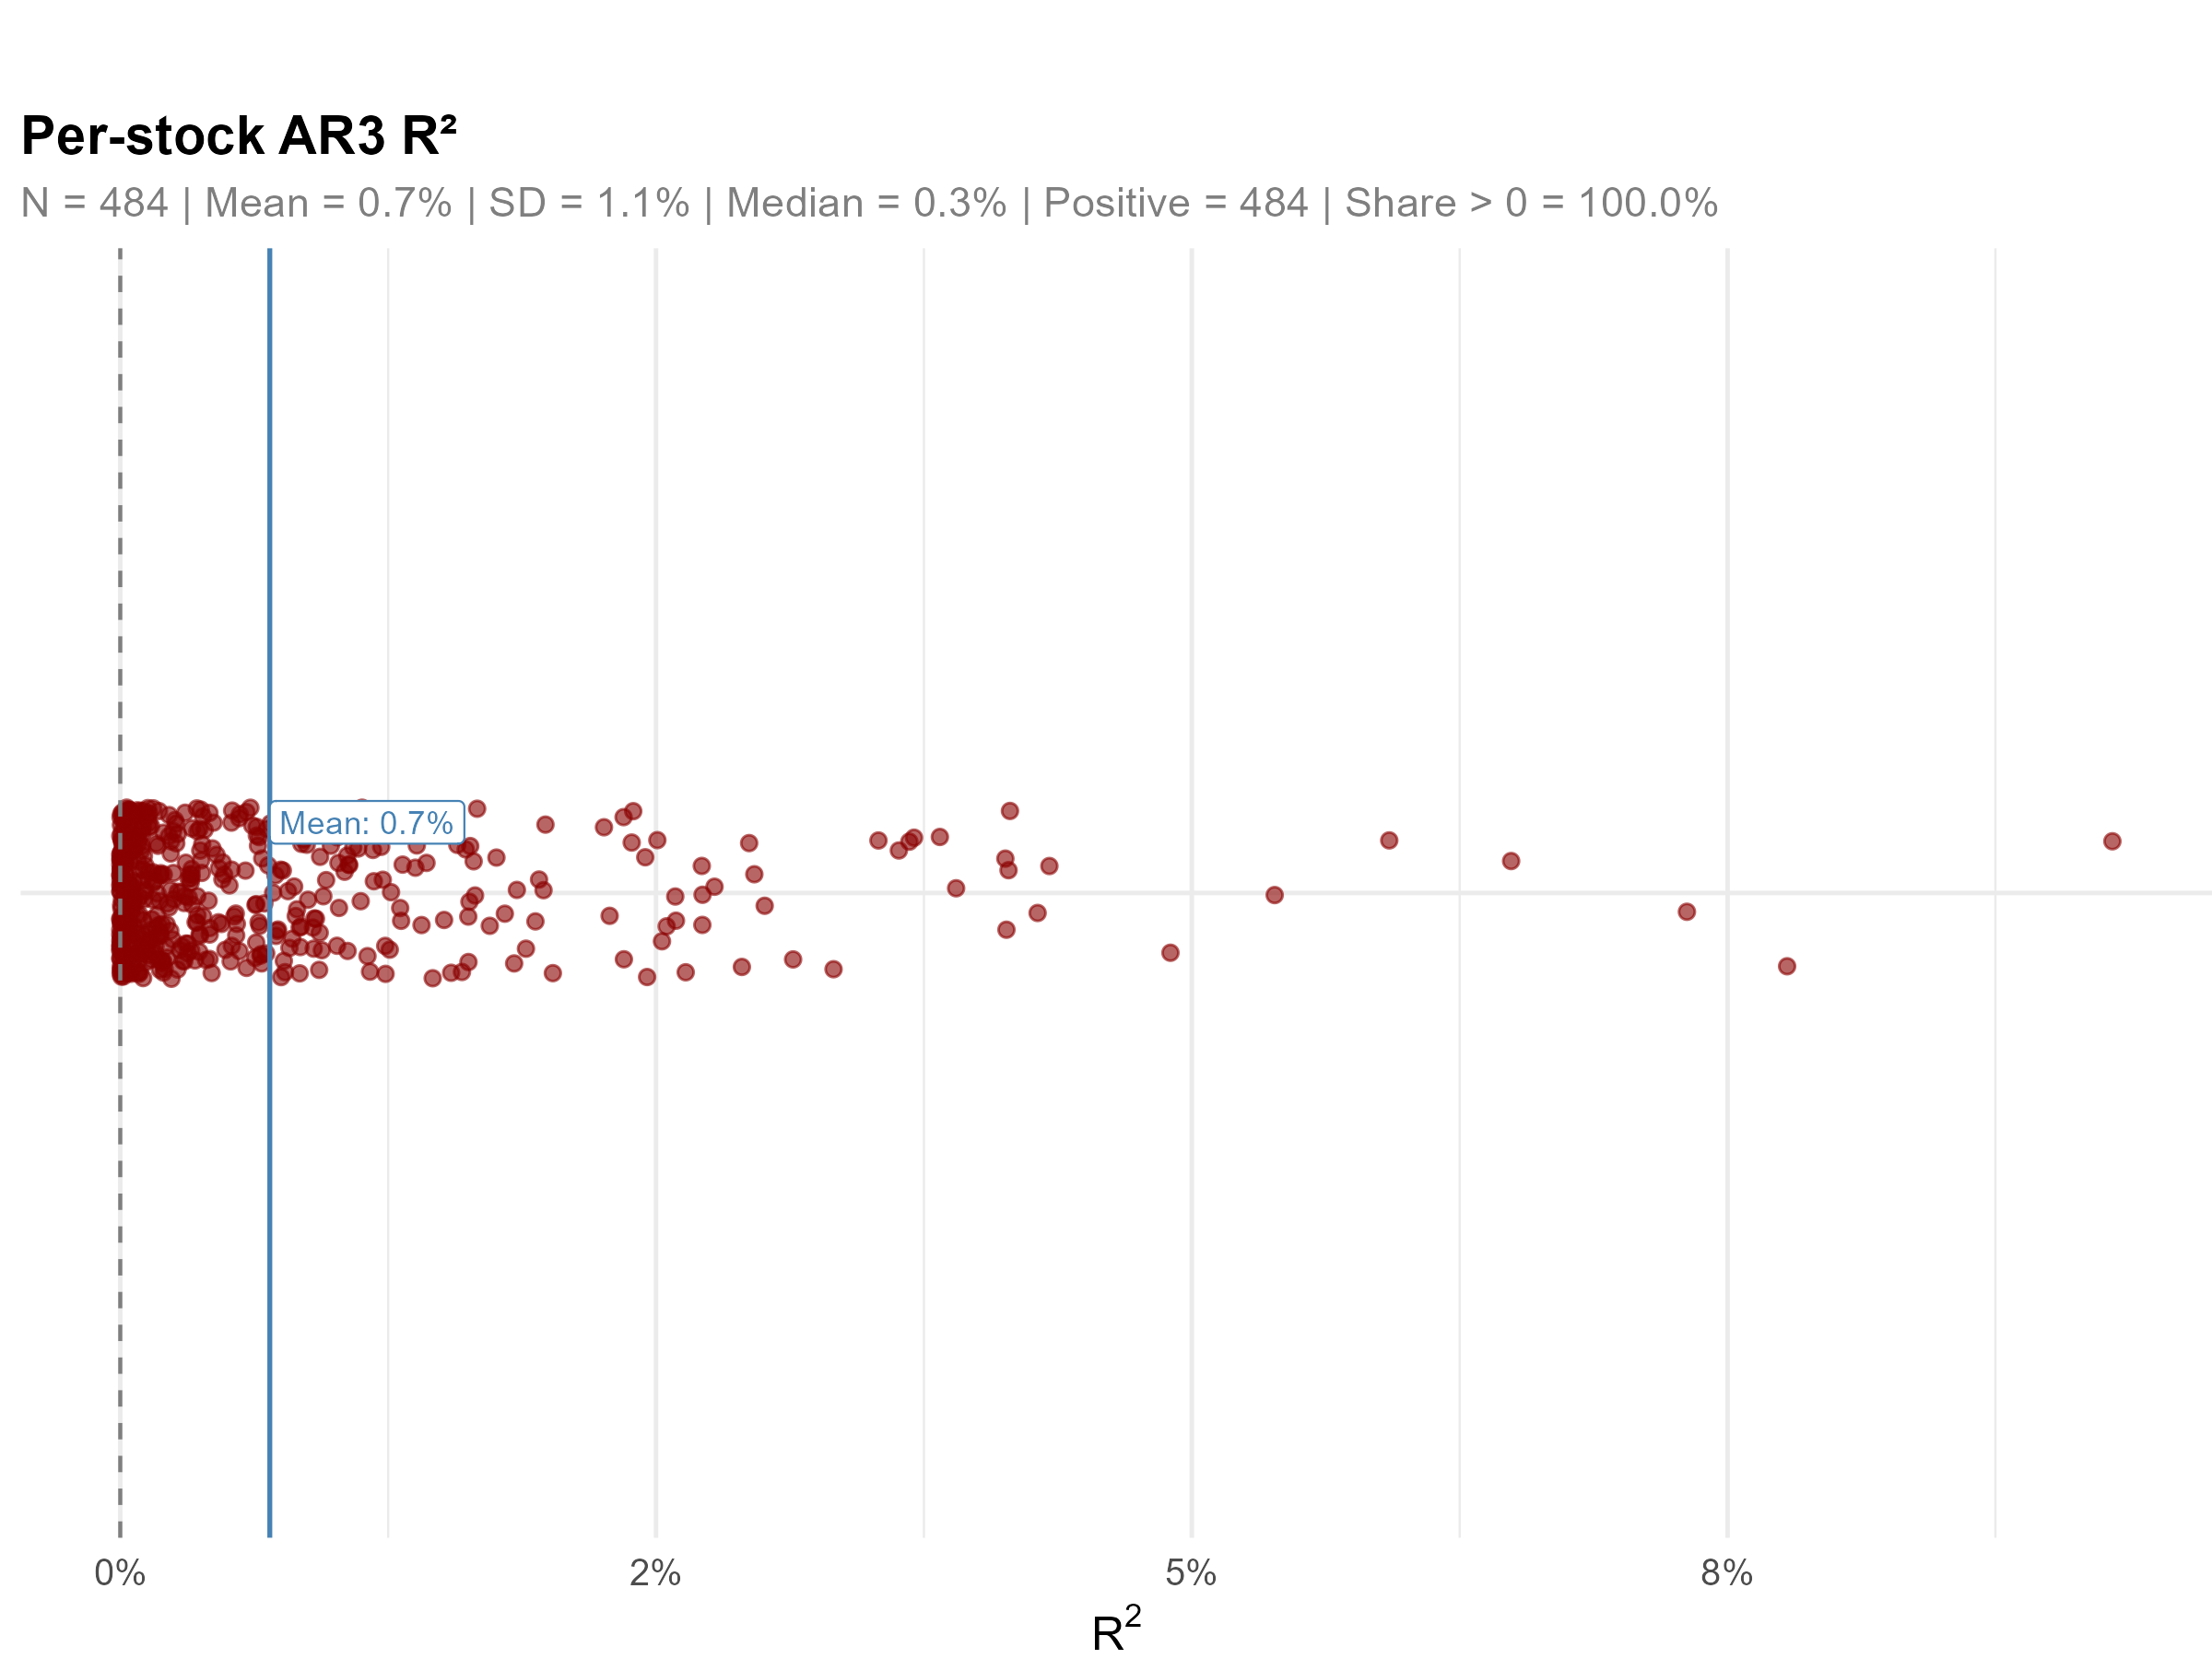
\includegraphics[width=0.45\textwidth]{ar3_r2_plot.png} 
    \caption{\(R^2\) values from regressions using AR(3) benchmark forecasts.}
    \label{fig:r2_oos_benchmark}  
\end{figure}

We next investigate the extent to which the information content of the LASSO and AR(3) forecasts overlaps. To this end, we re-estimate equation~\eqref{eq:r2_reg} including both predictors simultaneously. The results in Figure~\ref{fig:r2_oos_benchmar_lasso} show that the joint specification explains, on average, 2.8\% of the daily variation in returns. Figure~\ref{fig:r2_oos_benchmar_lasso_delta} reports the incremental change in \(R^2\) at the stock level.  

\begin{figure}[h!] % h! means "place here, if possible"
    \centering
    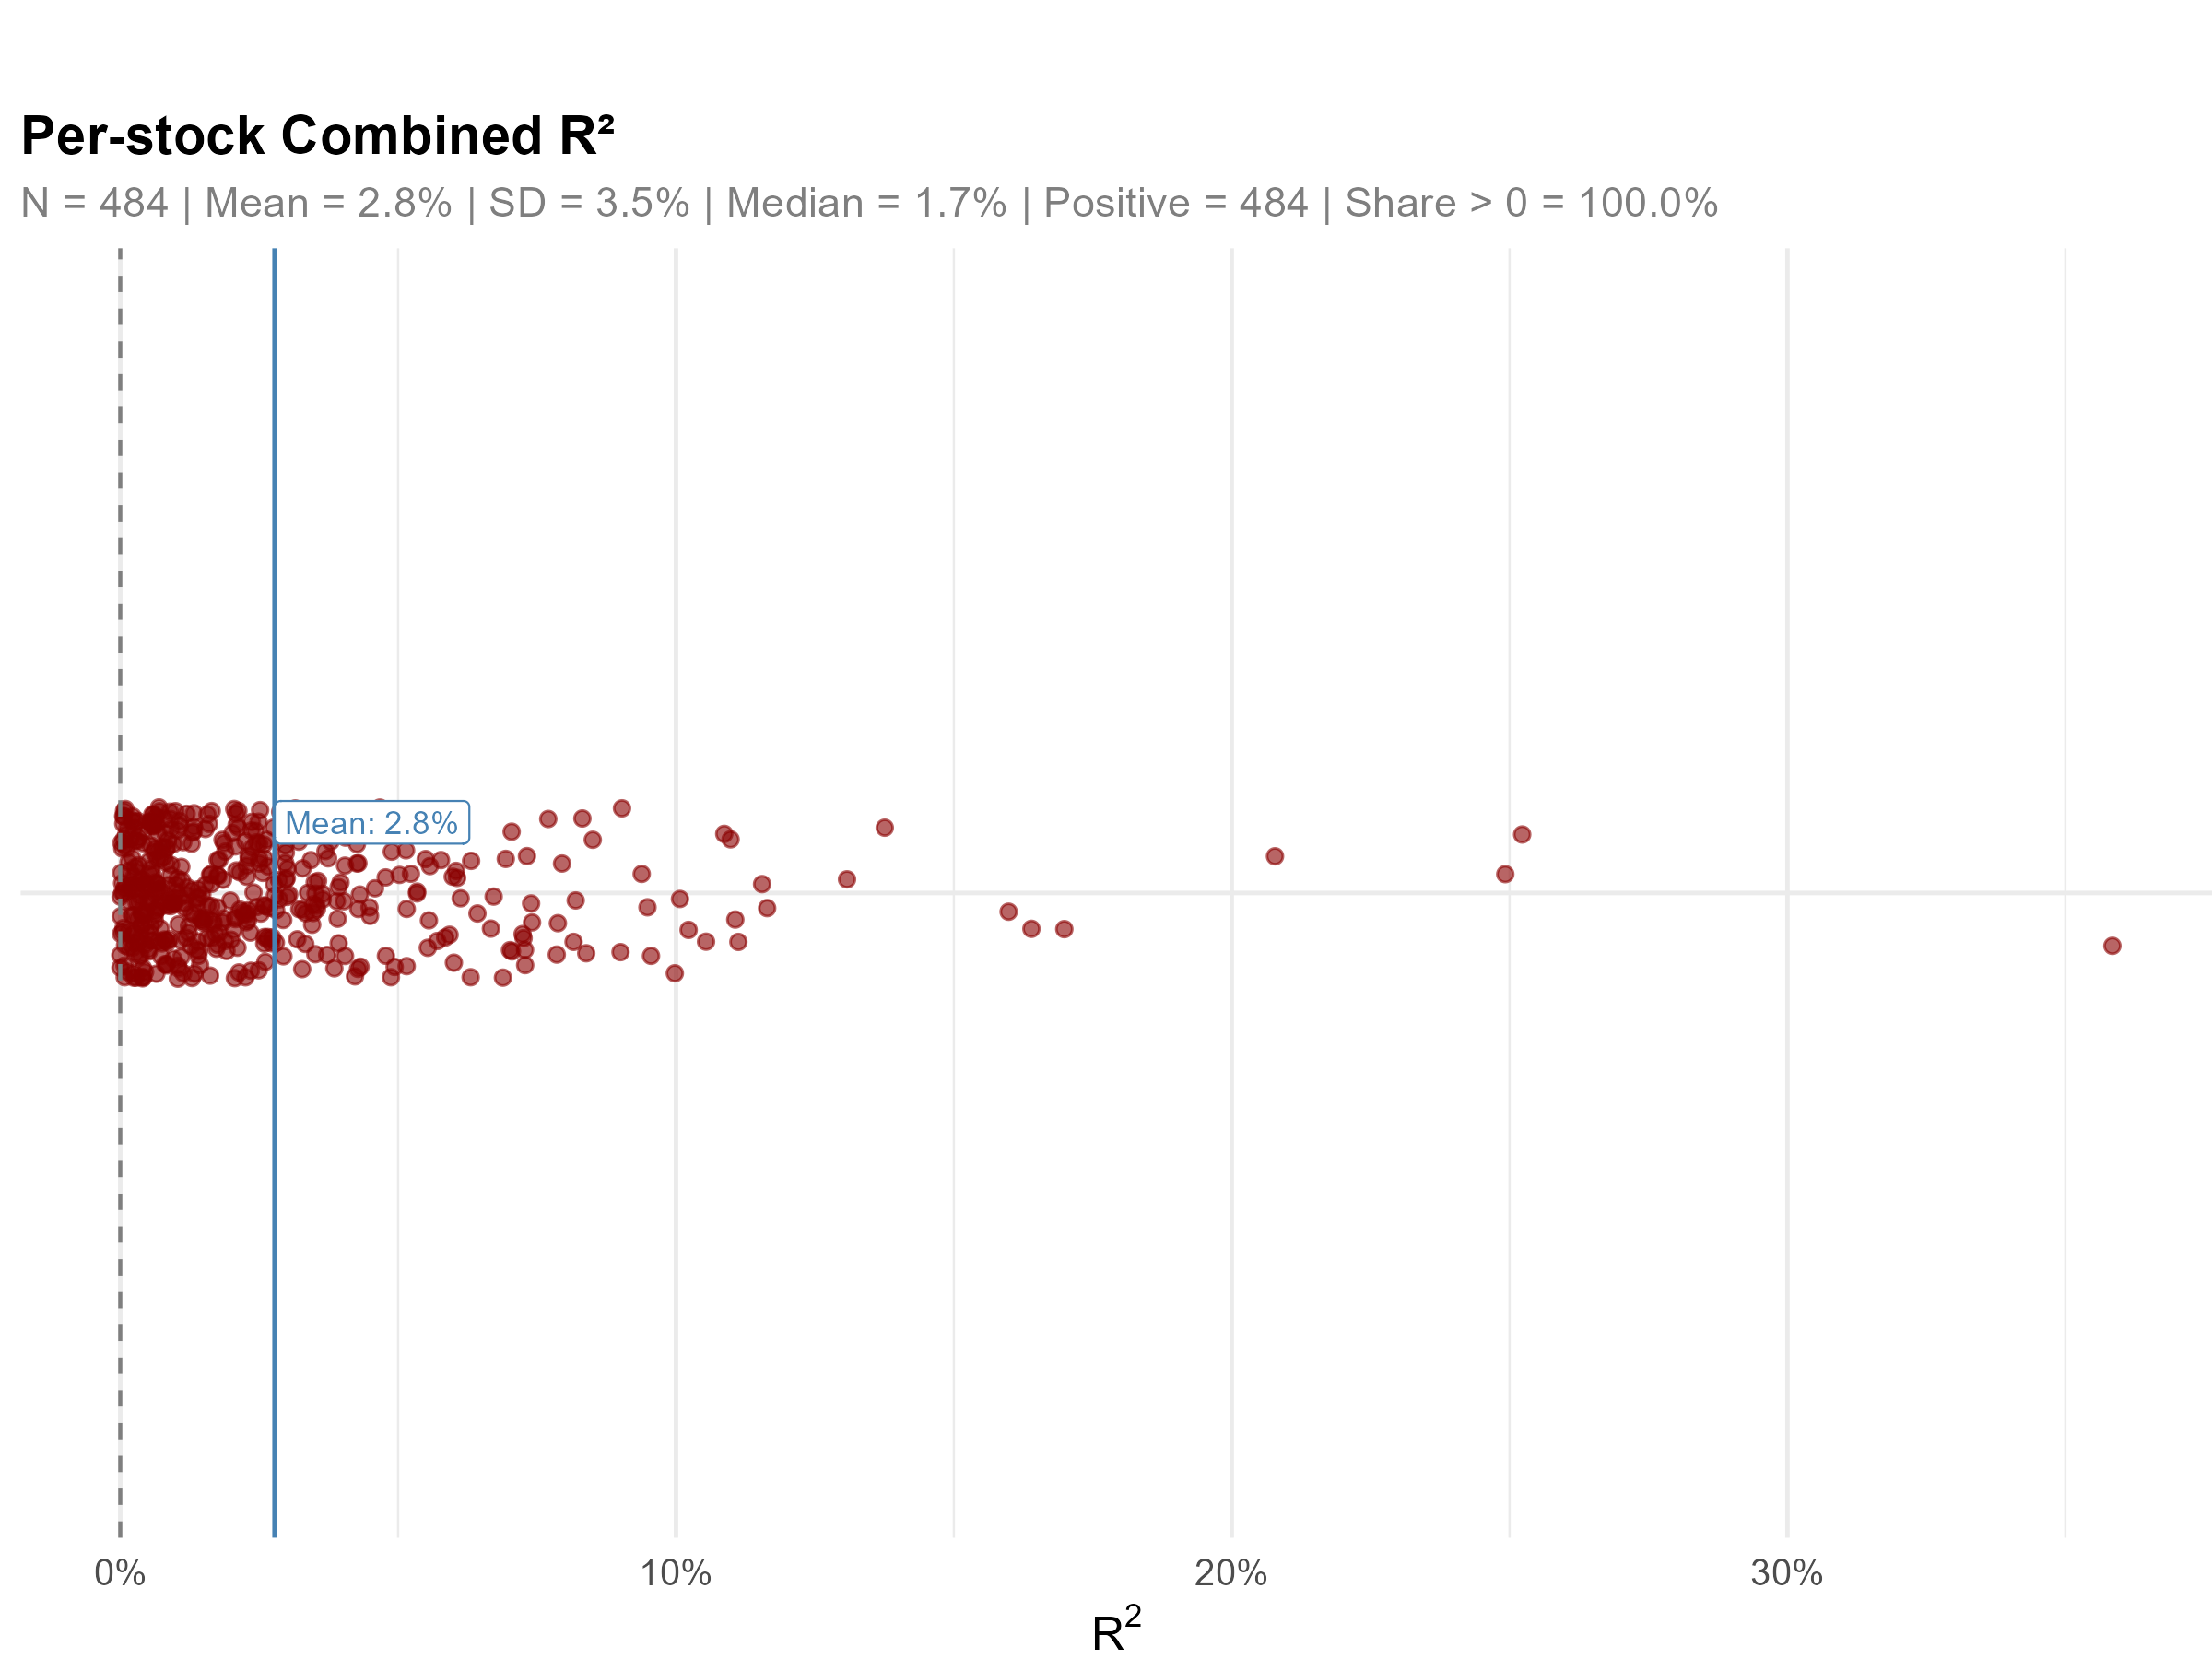
\includegraphics[width=0.45\textwidth]{combined_r2_plot.png} 
    \caption{\(R^2\) values from regressions using both LASSO and AR(3) forecasts.}
    \label{fig:r2_oos_benchmar_lasso} % Label for referencing
\end{figure}

\begin{figure}[h!] % h! means "place here, if possible"
    \centering
    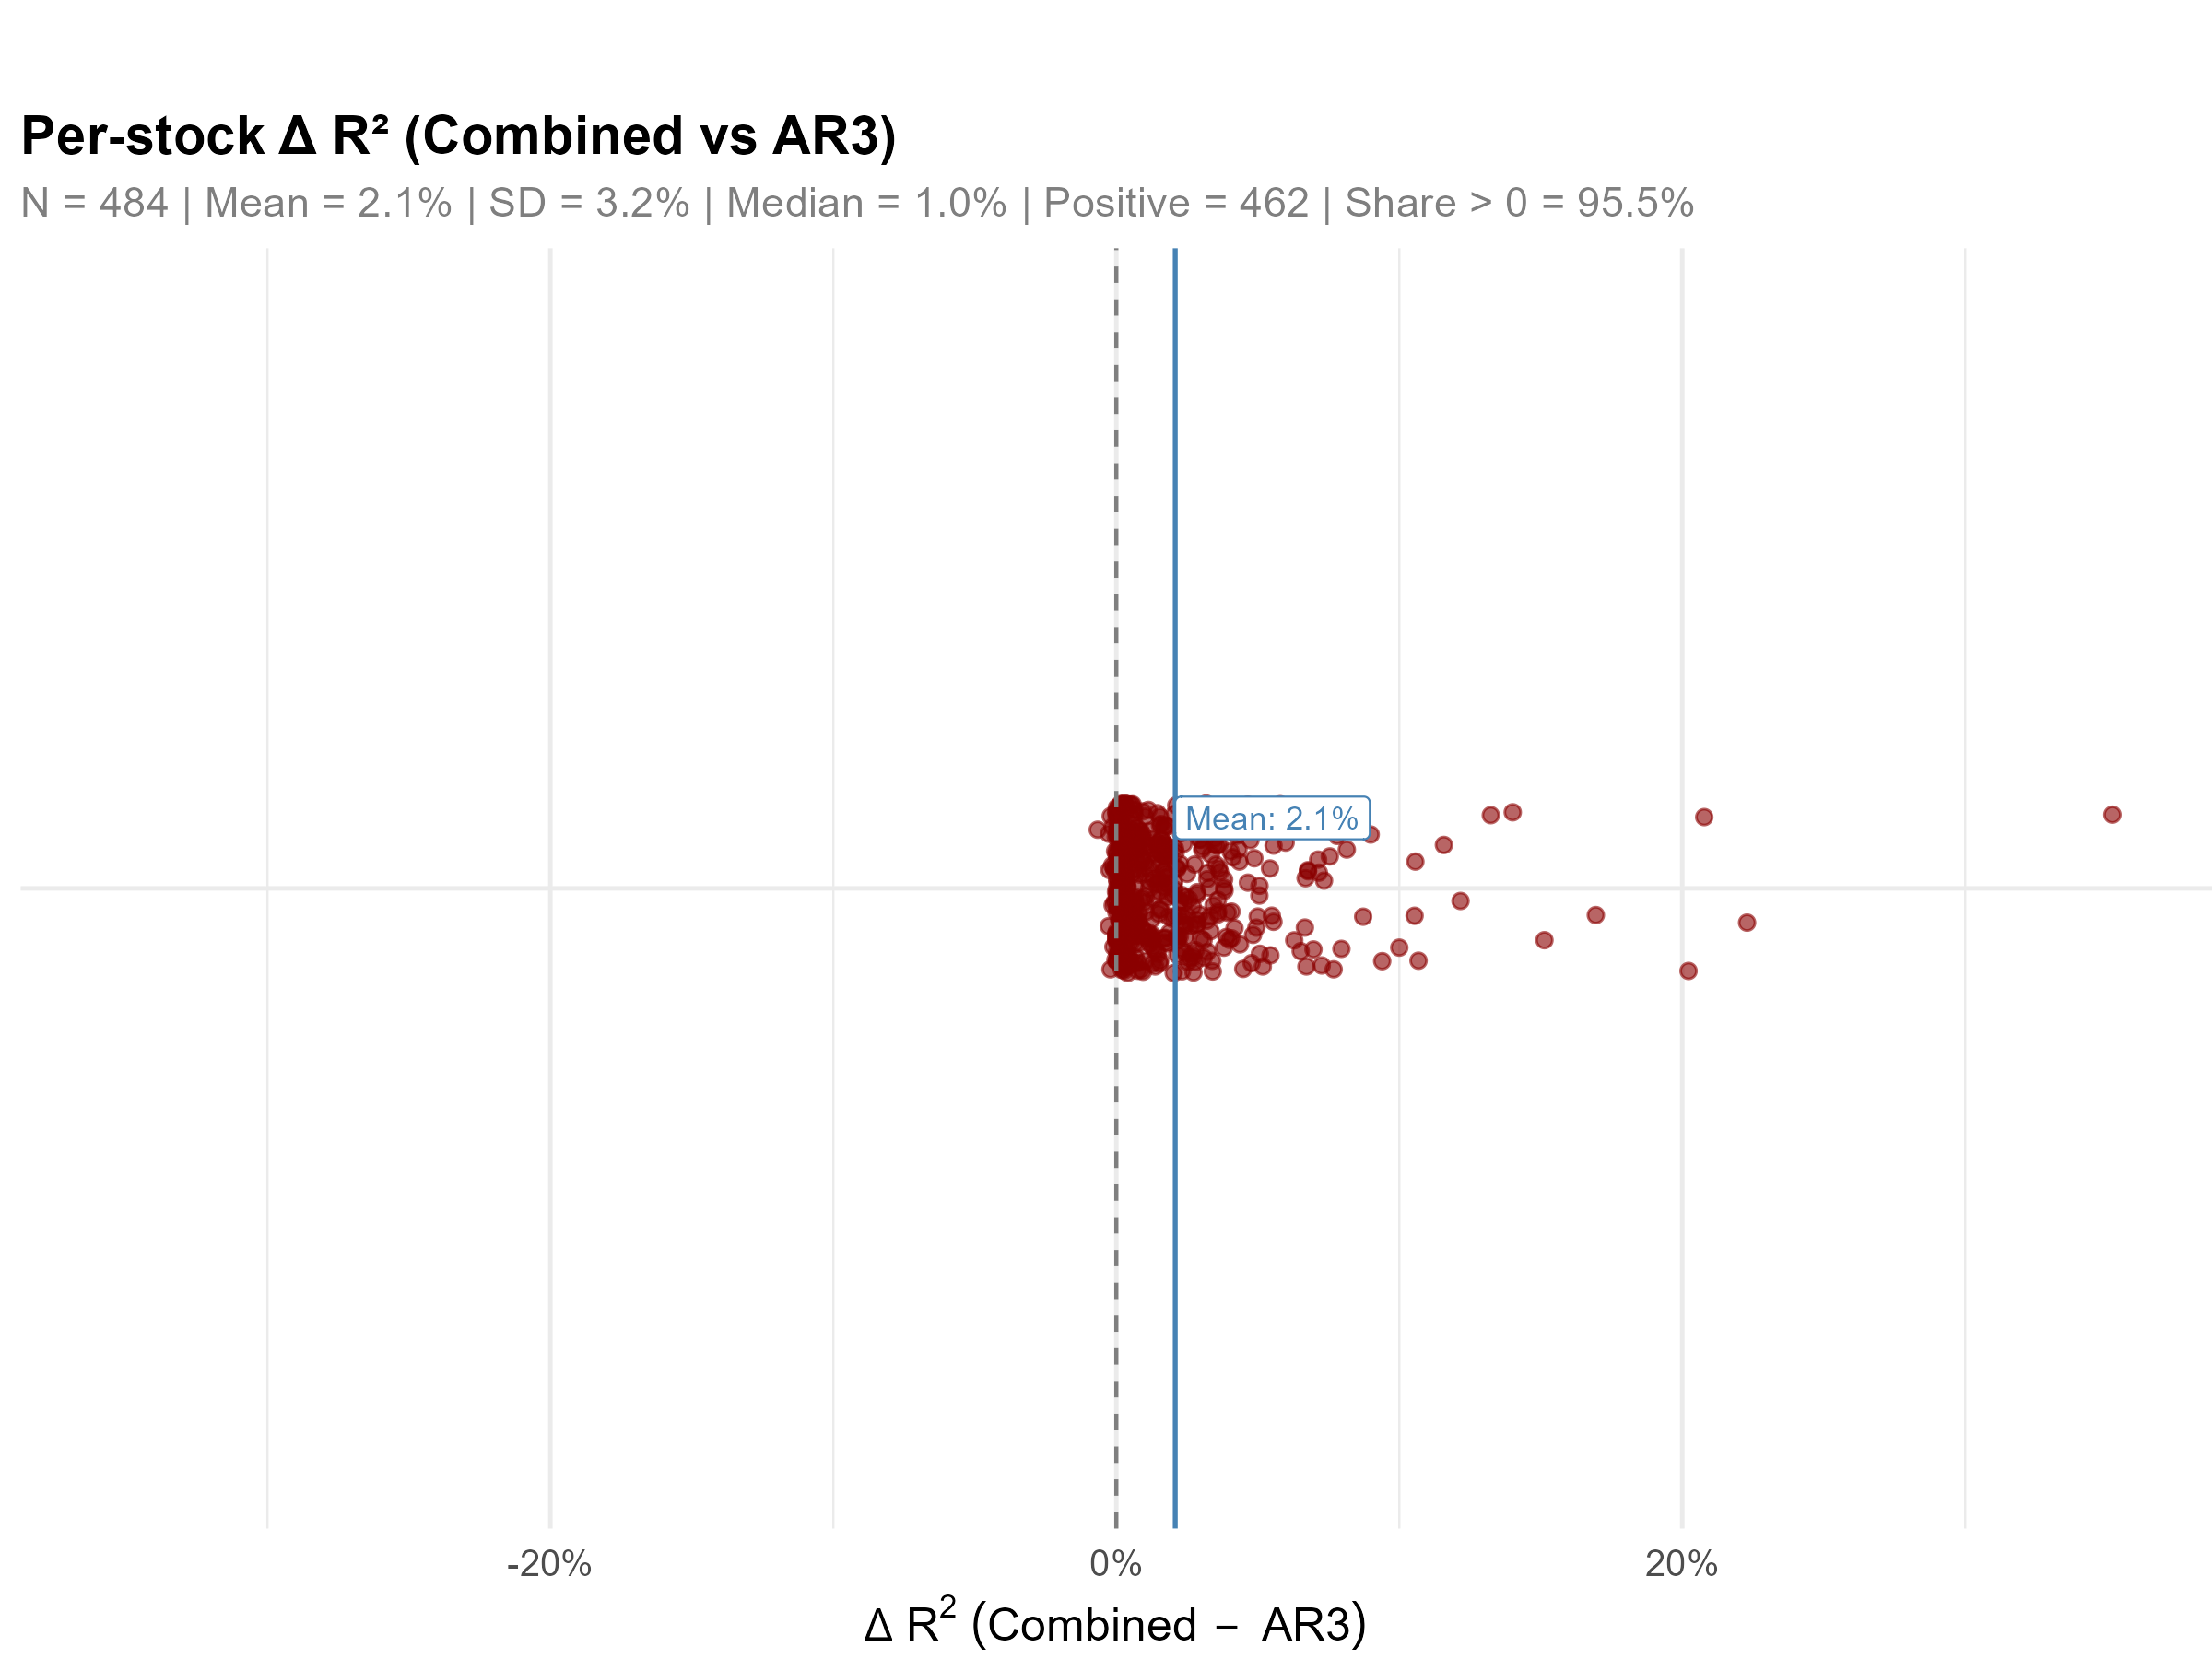
\includegraphics[width=0.45\textwidth]{delta_combined_ar3_r2_plot.png} 
    \caption{Change in $R^2$ from AR(3) only to AR(3) + LASSO.}
    \label{fig:r2_oos_benchmar_lasso_delta} % Label for referencing
\end{figure}


We next examine the time-series properties of the predictors selected by the LASSO. 
Figure~\ref{fig:persistence} plots the daily fraction of selected predictors that exhibit persistence. 
Persistence is assessed by estimating an AR(1) model for each selected predictor, using the same 
30-day rolling window employed in forecast construction: 
\begin{align}
r_{i,t} &= \alpha_i + \rho_i r_{i,t-1} + u_{i,t}, 
\label{eq:ar1_1}
\end{align}
where $r_{i,t}$ denotes the return of stock $i$ on day $t$, $\rho_i$ is the autoregressive 
coefficient, and $u_{i,t}$ is an error term. A predictor is classified as persistent if $\rho_i$ 
is statistically significant at the 5\% level. An identical specification is estimated for the 
news-based predictors, replacing returns with innovations in daily topic attention. 
The daily persistence share is defined as the ratio of predictors with significant $\rho_i$ to 
the total number of predictors selected across all forecasts on that day. Because predictors 
may be included in multiple forecasts, the same variable can contribute more than once to the 
daily share. 
On average, 7.2\% of predictors on a given day are persistent. This fraction fluctuates 
substantially over time and tends to increase during periods of heightened market volatility, 
such as the COVID-19 crash.
\begin{figure}[h!] % h! means "place here, if possible"
    \centering
    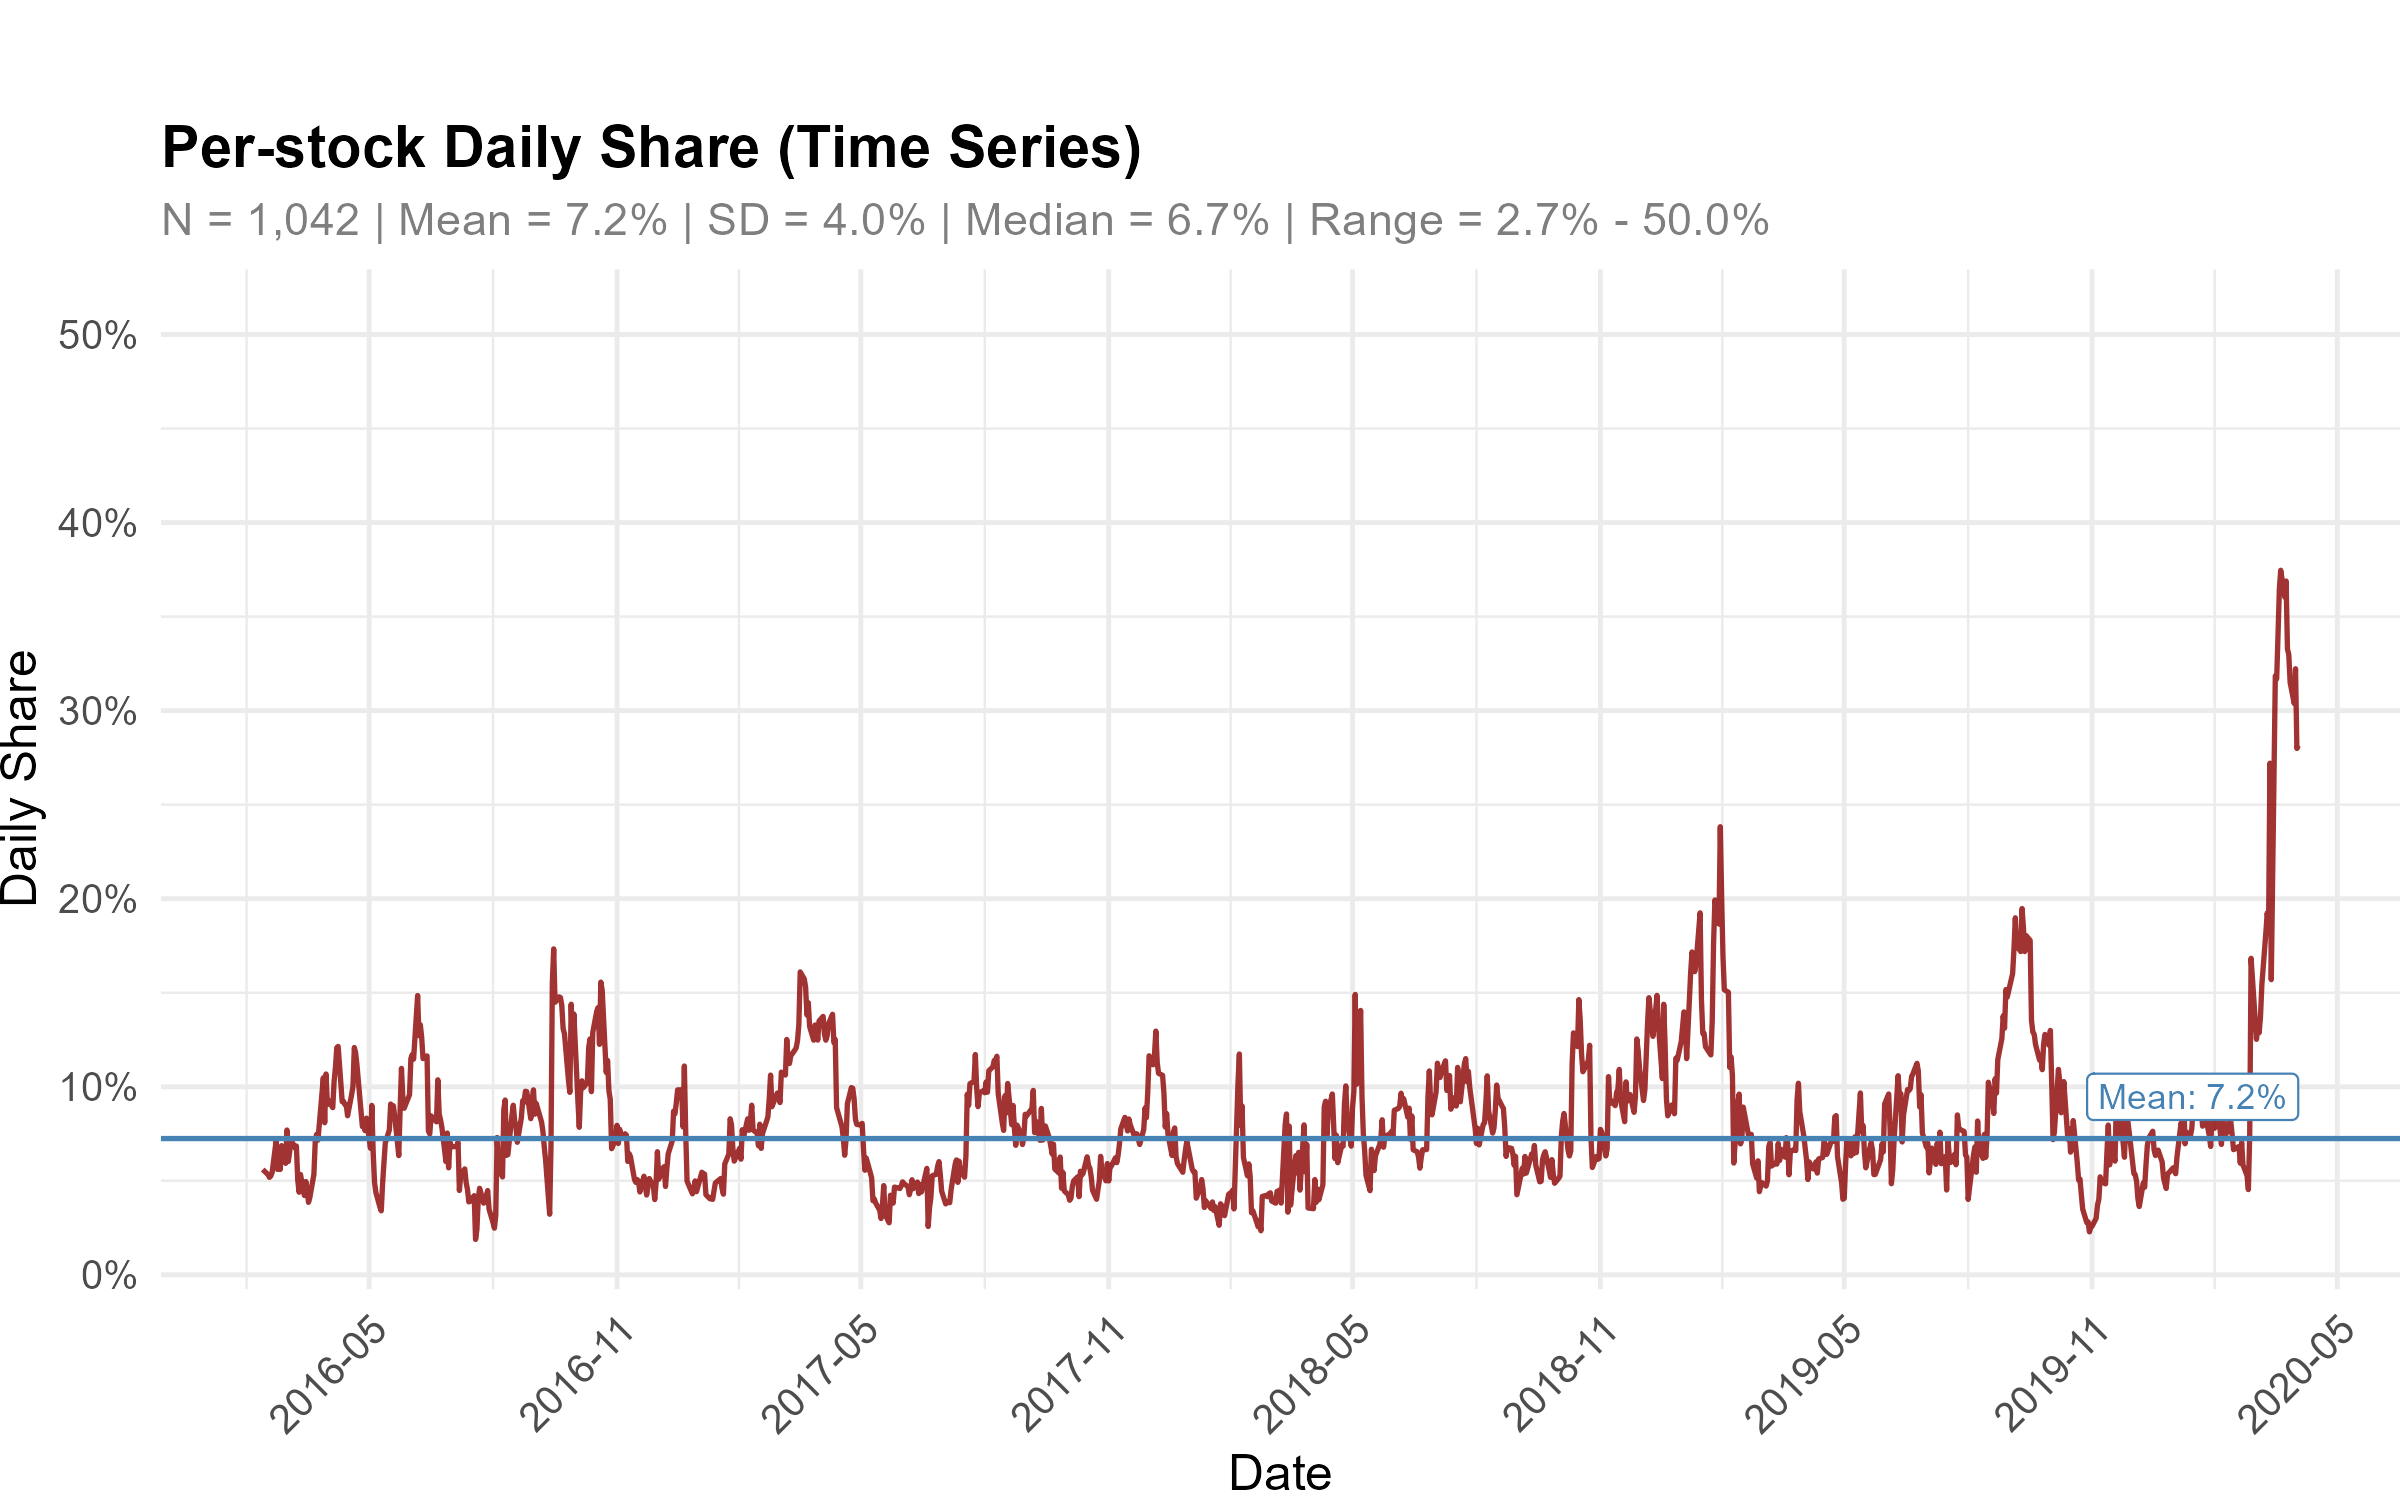
\includegraphics[width=0.45\textwidth]{daily_persistence_plot.png} 
    \caption{Daily share of Predictors selected by LASSO that are persistent.}
    \label{fig:persistence} % Label for referencing
\end{figure}

\printbibliography


\end{document}
